\documentclass[11pt]{article}

%\documentclass[aoas,preprint]{imsart}

%\RequirePackage[OT1]{fontenc}
%\RequirePackage{amsthm,amsmath,amssymb,caption,graphicx,subcaption}
%\RequirePackage{natbib}
%\RequirePackage[colorlinks,citecolor=blue,urlcolor=blue]{hyperref}





\usepackage{algorithm, alltt, amssymb, amsfonts, amsmath, caption, color,
    fancyhdr, graphicx, mathrsfs, moreverb, natbib, setspace, subcaption, tikz,
    titling, ulem, verbatim}
\usepackage[noend]{algpseudocode}
\renewcommand{\algorithmicrequire}{\textbf{Input:}}
\renewcommand{\algorithmicensure}{\textbf{Output:}}

\addtolength{\oddsidemargin}{-.875in}
\addtolength{\evensidemargin}{-.875in}
\addtolength{\textwidth}{1.75in}
\addtolength{\topmargin}{-.875in}
\addtolength{\textheight}{1.75in}

\newtheorem{proposition}{Proposition}

\def\A{\mathcal A}\def\B{\mathcal B}\def\C{\mathcal C}\def\D{\mathcal D}
\def\E{\mathcal E}\def\F{\mathcal F}\def\G{\mathcal G}\def\I{\mathcal I}
\def\J{\mathcal J}\def\L{\mathcal L}\def\M{\mathcal M}\def\N{\mathcal N}
\def\O{\mathcal O}\def\P{\mathcal P}\def\Q{\mathcal Q}\def\R{\mathcal R}
\def\S{\mathcal S}\def\T{\mathcal T}\def\W{\mathcal W}\def\V{\mathcal V}
\def\X{\mathcal X}\def\Y{\mathcal Y}\def\Z{\mathcal Z}
\def\mI{\mathbb I}\def\mN{\mathbb N}\def\mR{\mathbb R}\def\mS{\mathbb S}
\def\bE{{\bf E}}
\def\bx{{\bf x}}

\def\bam{\hspace{1cm}$\blacksquare$}\def\pow{\hspace{1cm}\blacksquare}
\def\prob{\mbox{\bf prob}}\def\tr{\mbox{\bf tr}}
\def\l{\left}\def\r{\right}\def\lf{\lfloor}\def\rf{\rfloor}
\def\un{\underline}
\def\theat{\theta}\def\lambad{\lambda}\def\lamda{\lambda}
\def\minimize{\mbox{minimize}\hspace{4mm}}
\def\maximize{\mbox{maximize}\hspace{4mm}}
\def\subjectto{\mbox{subject to}\hspace{4mm}}

\title{True wOBA: Estimation of true talent level for batters}
\author{Scott Powers and Eli Shayer}

\begin{document}

\maketitle

\section{Introduction}

Batting statistics at the play-by-play level are a solved problem. Thanks to
weighted on-base average (wOBA), we know the marginal run value of each
possible outcome of a plate appearance (PA) given a specific run environment
\citep{TheBook}. But player evaluation is a two-step process: (1) estimate the
value of each outcome and (2) estimate the frequency with which the player
produces each outcome. Relative to the first step, sabermetric literature has
paid little attention to the second step. In this paper we develop a model for
estimating batters' true talent level for wOBA while simultaneously adjusting
for sample size, park effects and opponent quality.

\section{Review of related work}

Several recent papers \citep{Brown08, Null09, Neal.etal10, Albert15} have
proposed methods for estimating or predicting batting statistics. In contrast
with projection systems, these methods implicitly assume that players' skills
remain constant between training sample and test sample (as opposed to
modeling the aging of skills). True wOBA differs from the above by adjusting
for park effects and quality of opposition. Deserved Run Average
\citep{Judge15} uses a very similar model to True wOBA to estimate pitchers'
component skills (e.g. strikeout rate). True wOBA could accurately be described
as a version of DRA for batters.

\section{Research methodology}

\subsection{Data}

Our dataset, from Retrosheet, comprises all plate appearances (PAs) from the
2015 MLB regular season. For each plate appearance (PA) we have the identity
and handedness of the batter and pitcher, the ballpark at which the PA took
place, and the result of the PA.

\subsection{Methods}

True wOBA is based on a ridge regressed multinomial Rasch model which models
the probability of each outcome of an at-bat as a function of the difference
between the batter's propensity for producing the outcome and the pitcher's
propensity for preventing the outcome, with adjustments for ballpark and
handedness.

\section{Anticipated results}

We split the data into a training sample and a test sample, using
the training sample to estimate batters' skills and the test sample to evaluate
these estimates. Our results compare the performance of True wOBA with both
naive estimators and the state of the art. Additionally, we present the impact
of sample size and BABIP (e.g. see figure below) on the difference between
observed wOBA and True wOBA. Intermediate results compare an opponent-agnostic
special case of True wOBA with standard regression to the mean, thus
illustrating the relationship between the two.

\begin{center}
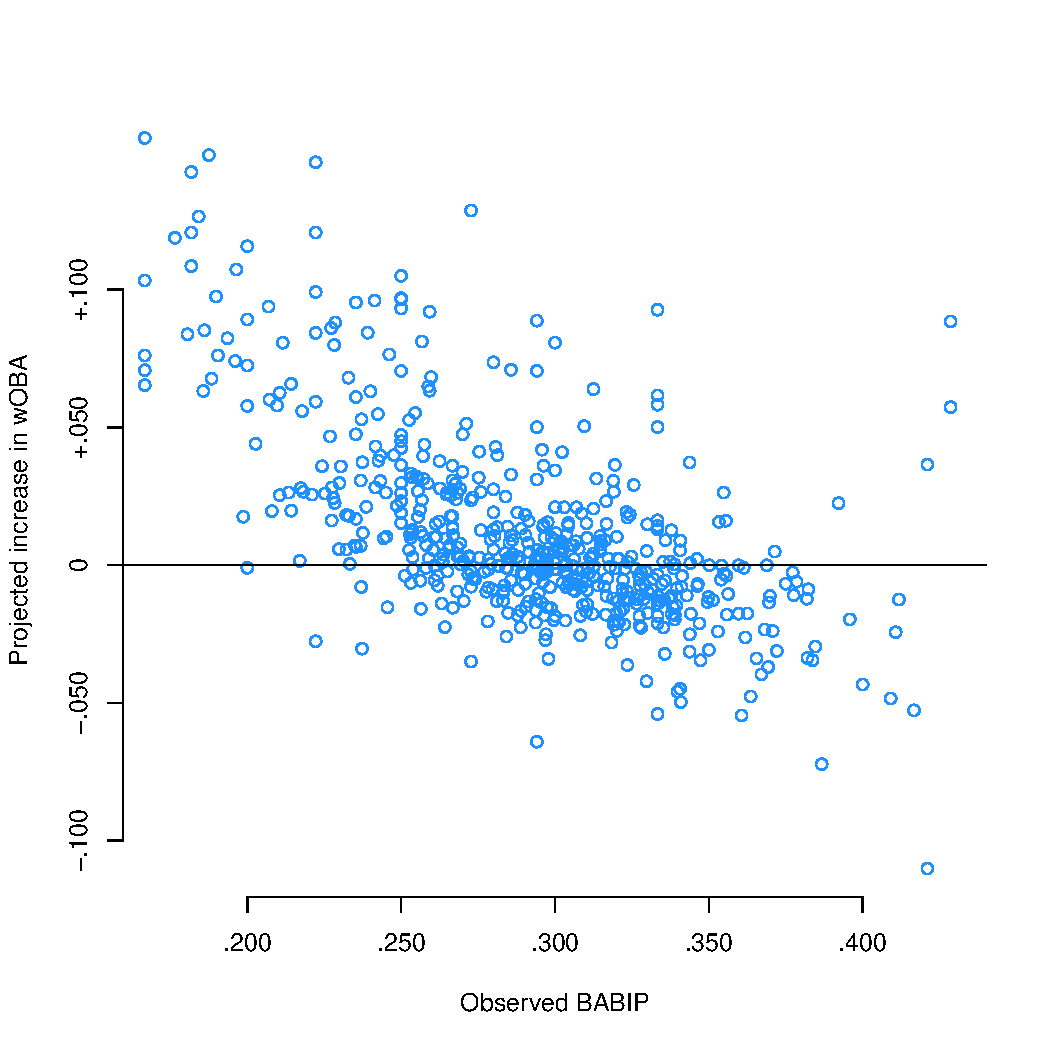
\includegraphics[width = 0.4\textwidth]{../figs/woba-v-babip.pdf}
\end{center}

\section{Expected contribution}

Because we cannot observe an infinite sequence of plate appearances for a
batter, we will never know the true probability with which he produces each
outcome. Major League clubs can benefit from making the most out of a finite
sample of data when learning the batters' skills, which has immediate
applications to lineup and roster decisions. Baseball writers can also benefit
from understanding how to quantitatively adjust for small sample sizes and
low/high BABIPs, instead of qualitatively citing those as reasons that a
batter's wOBA may not be an accurate reflection of his abilities.

\bibliographystyle{apalike}
\bibliography{baseball}

\end{document}
